\chapter{場景佈置}
\section{機器人}
\begin{figure}[hbt!]
\begin{center}
\label{各自機器人圖}
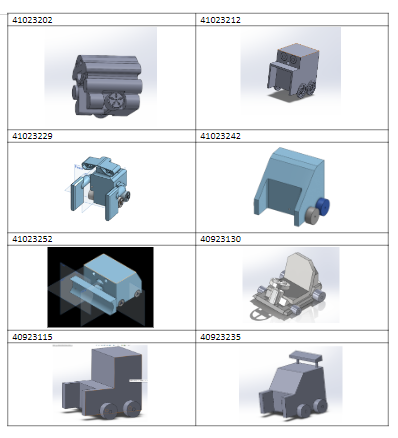
\includegraphics[width=\textwidth]{各自機器人圖}
\caption{\Large 機器人繪製}
\end{center}
\end{figure}
\newpage

\section{記分板}
\begin{figure}[hbt!]
\begin{center}
\label{記分板}
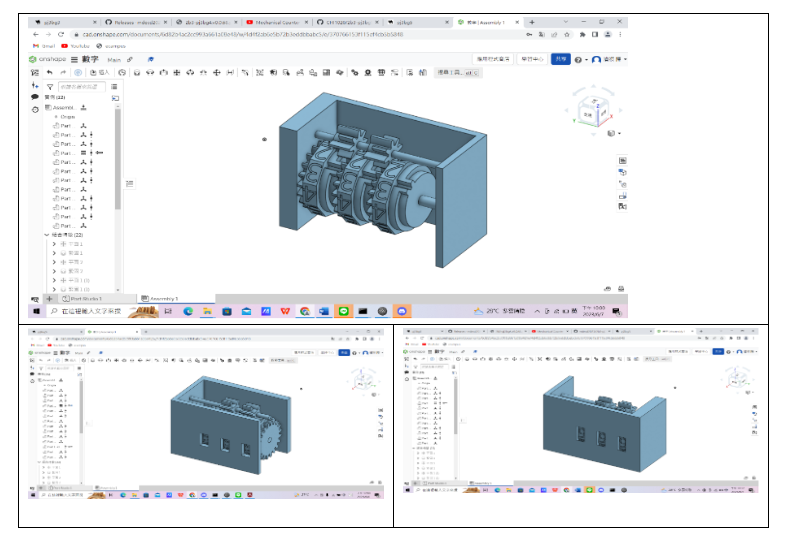
\includegraphics[width=\textwidth]{記分板}
\caption{\Large 記分板繪製}
\end{center}
\end{figure}
\newpage

\section{場景}
\begin{figure}[hbt!]
\begin{center}
\label{場景}
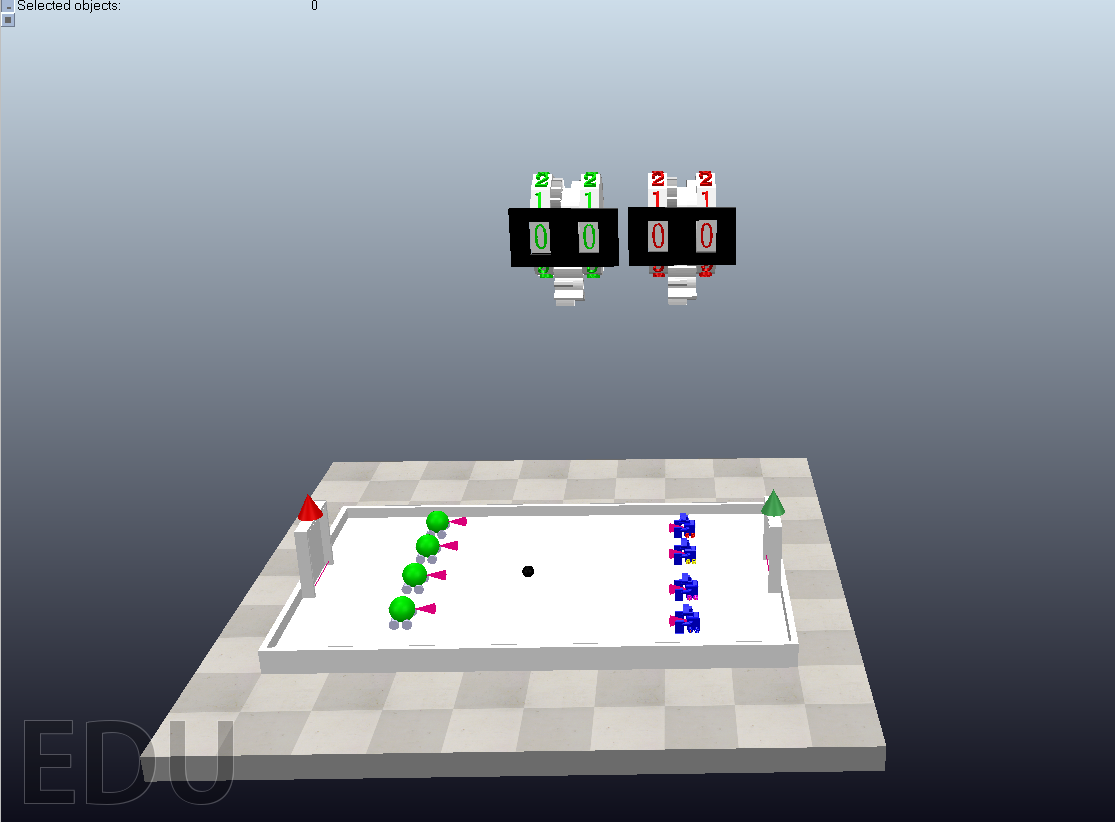
\includegraphics[width=\textwidth]{場景}
\caption{\Large 場景}
\end{center}
\end{figure}
\newpage
